\documentclass{beamer}

\usepackage{framed}
\usepackage{graphicx}

\usepackage{amsmath}

\begin{document}
%================================================================================== %
\section{How it works}
\begin{frame}[fragile]
	\Large
\frametitle{Basic Premise}
\begin{itemize}
\item Making plots is a very repetive: draw this line, add these colored points, then add these, etc. 
\item Instead of re-using the same code over and over, \texttt{ggplot} implements them using a high-level but very expressive API.
\item The result is less time spent creating your charts, and more time interpreting what they mean.
\end{itemize}

\end{frame}
%================================================================================== %
\begin{frame}[fragile]
	\Large
	\begin{itemize}
\item \texttt{ggplot} is not a good fit for people trying to make highly customized data visualizations. 
\item While you can make some very intricate, great looking plots, \texttt{ggplot} sacrafices highly customization in favor of generall doing "what you'd expect".
	\end{itemize}

\end{frame}
%================================================================================== %
\begin{frame}[fragile]
\frametitle{Data}
\Large
\begin{itemize}
\item ggplot has a symbiotic relationship with pandas. 
\item If you're planning on using ggplot, it's best to keep your data in DataFrames. 
\item Think of a DataFrame as a tabular data object. 
\item For example, let's look at the diamonds dataset which ships with ggplot.
\end{itemize}
\end{frame}
%================================================================================== %
\begin{frame}[fragile]
\begin{framed}
	\begin{verbatim}
from ggplot import *
diamonds.head()
\end{verbatim}
\end{framed}
\begin{figure}
\centering
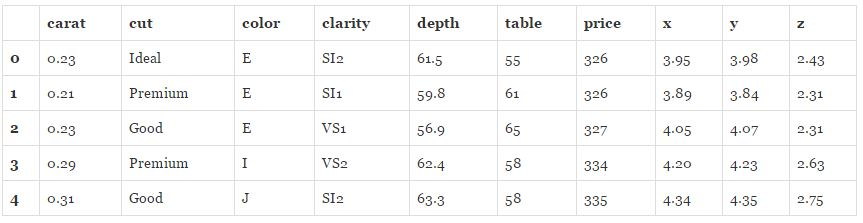
\includegraphics[width=1.1\linewidth]{diamondsdata}

\end{figure}

\end{frame}	
%================================================================================== %
\begin{frame}[fragile]
\frametitle{Aesthetics}
\Large
\noindent \textbf{Aesthetics}
\begin{itemize}
\item Aesthetics describe how your data will relate to your plots.
\item Some common aesthetics are: x, y, and color. \item Aesthetics are specific to the type of plot (or layer) you're adding to your visual. 
\item For example, a scatterplot (\texttt{geom\_point}) and a line (\texttt{geom\_line}) will share x and y, but only a line chart has a linetype aesthetic.
\end{itemize}


%For more information about which geoms have which aesthetics, see the DOCS SECTION.
\end{frame}
%================================================================================== %
\begin{frame}[fragile]
\frametitle{Layers}
\Large
\noindent \textbf{Layers}
\begin{itemize}
\item ggplot lets you combine or add different types of visualization components (or layers) together. 
%\item I think this is easiest to understand with an example.
\item The command ggplot does not actually create any plot, rather it prepares a ``blank canvas" for further plotting 
\end{itemize}

\end{frame}
%================================================================================== %
\begin{frame}[fragile]
Start with a blank canvas.
\begin{framed}
\begin{verbatim}
p = ggplot(aes(x="date", y="beef"), data=meat)
p
\end{verbatim}
\end{framed}
\begin{figure}
\centering
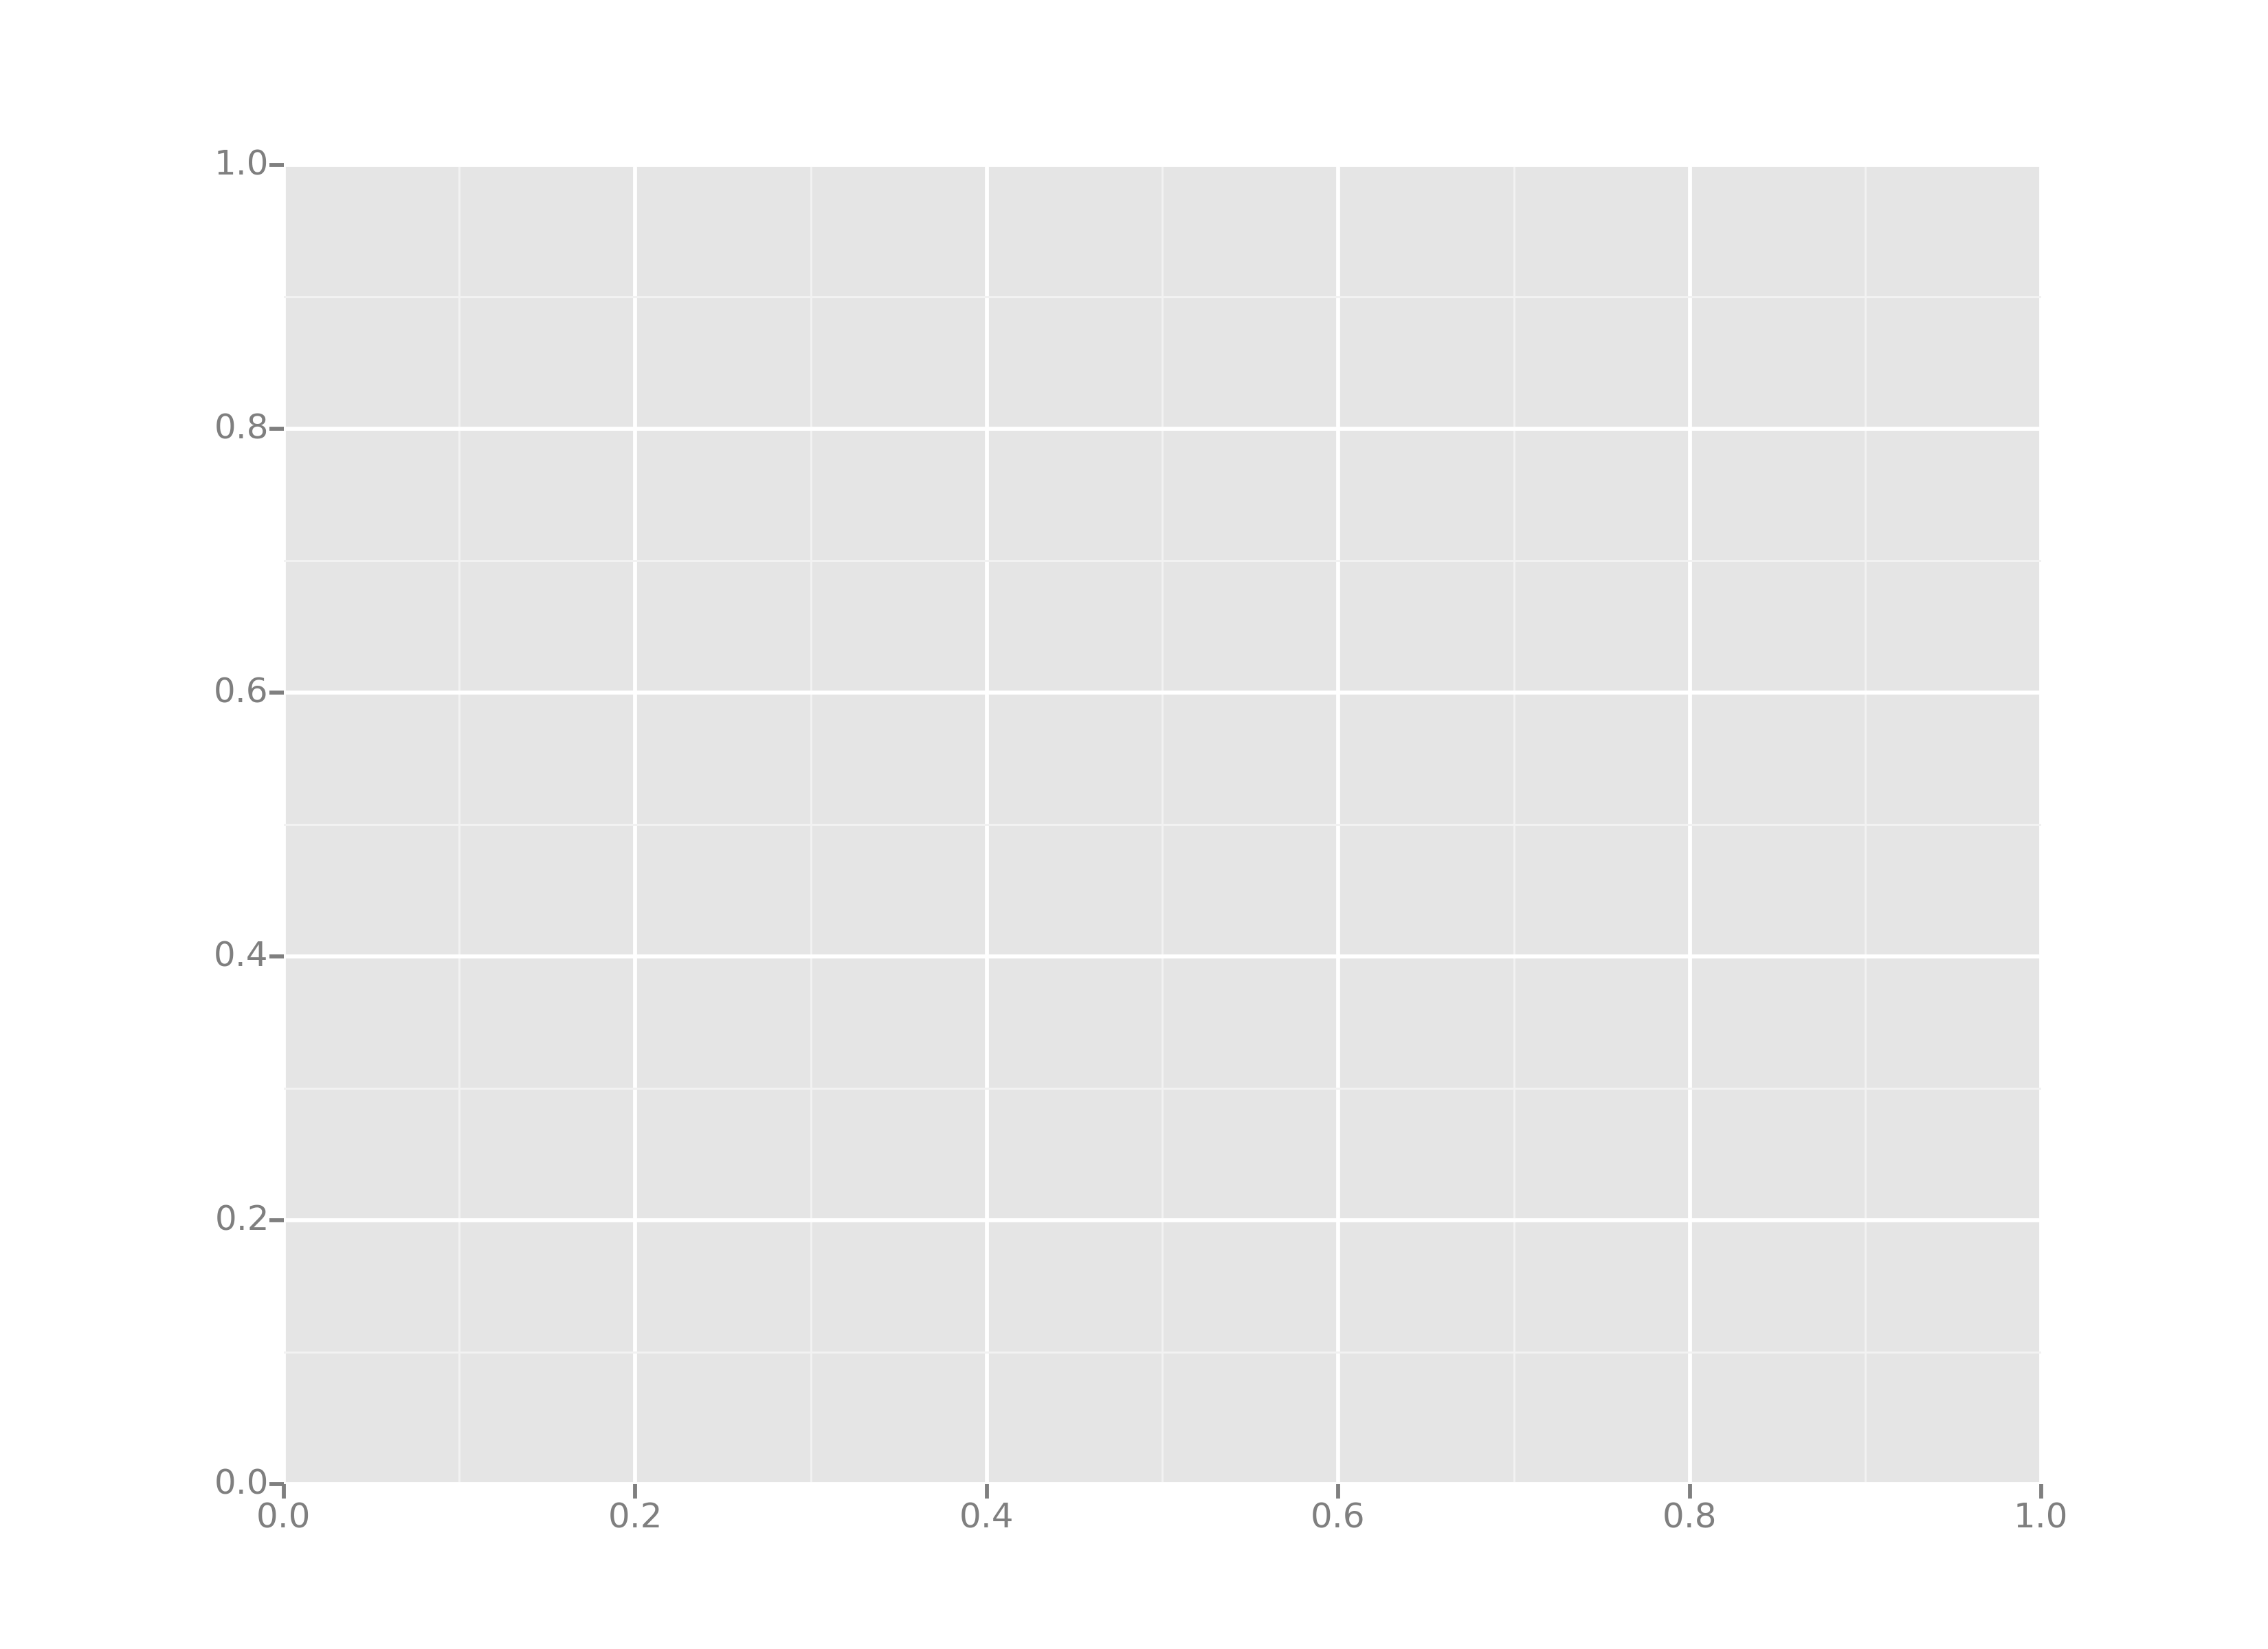
\includegraphics[width=0.7\linewidth]{Layers1}
\caption{}
\label{fig:Layers1}
\end{figure}

\end{frame}
%================================================================================== %
\begin{frame}[fragile]
	Add some points.
	\begin{framed}
		\begin{verbatim}
		p + geom_point()
		\end{verbatim}
	\end{framed}
	\begin{figure}
		\centering
		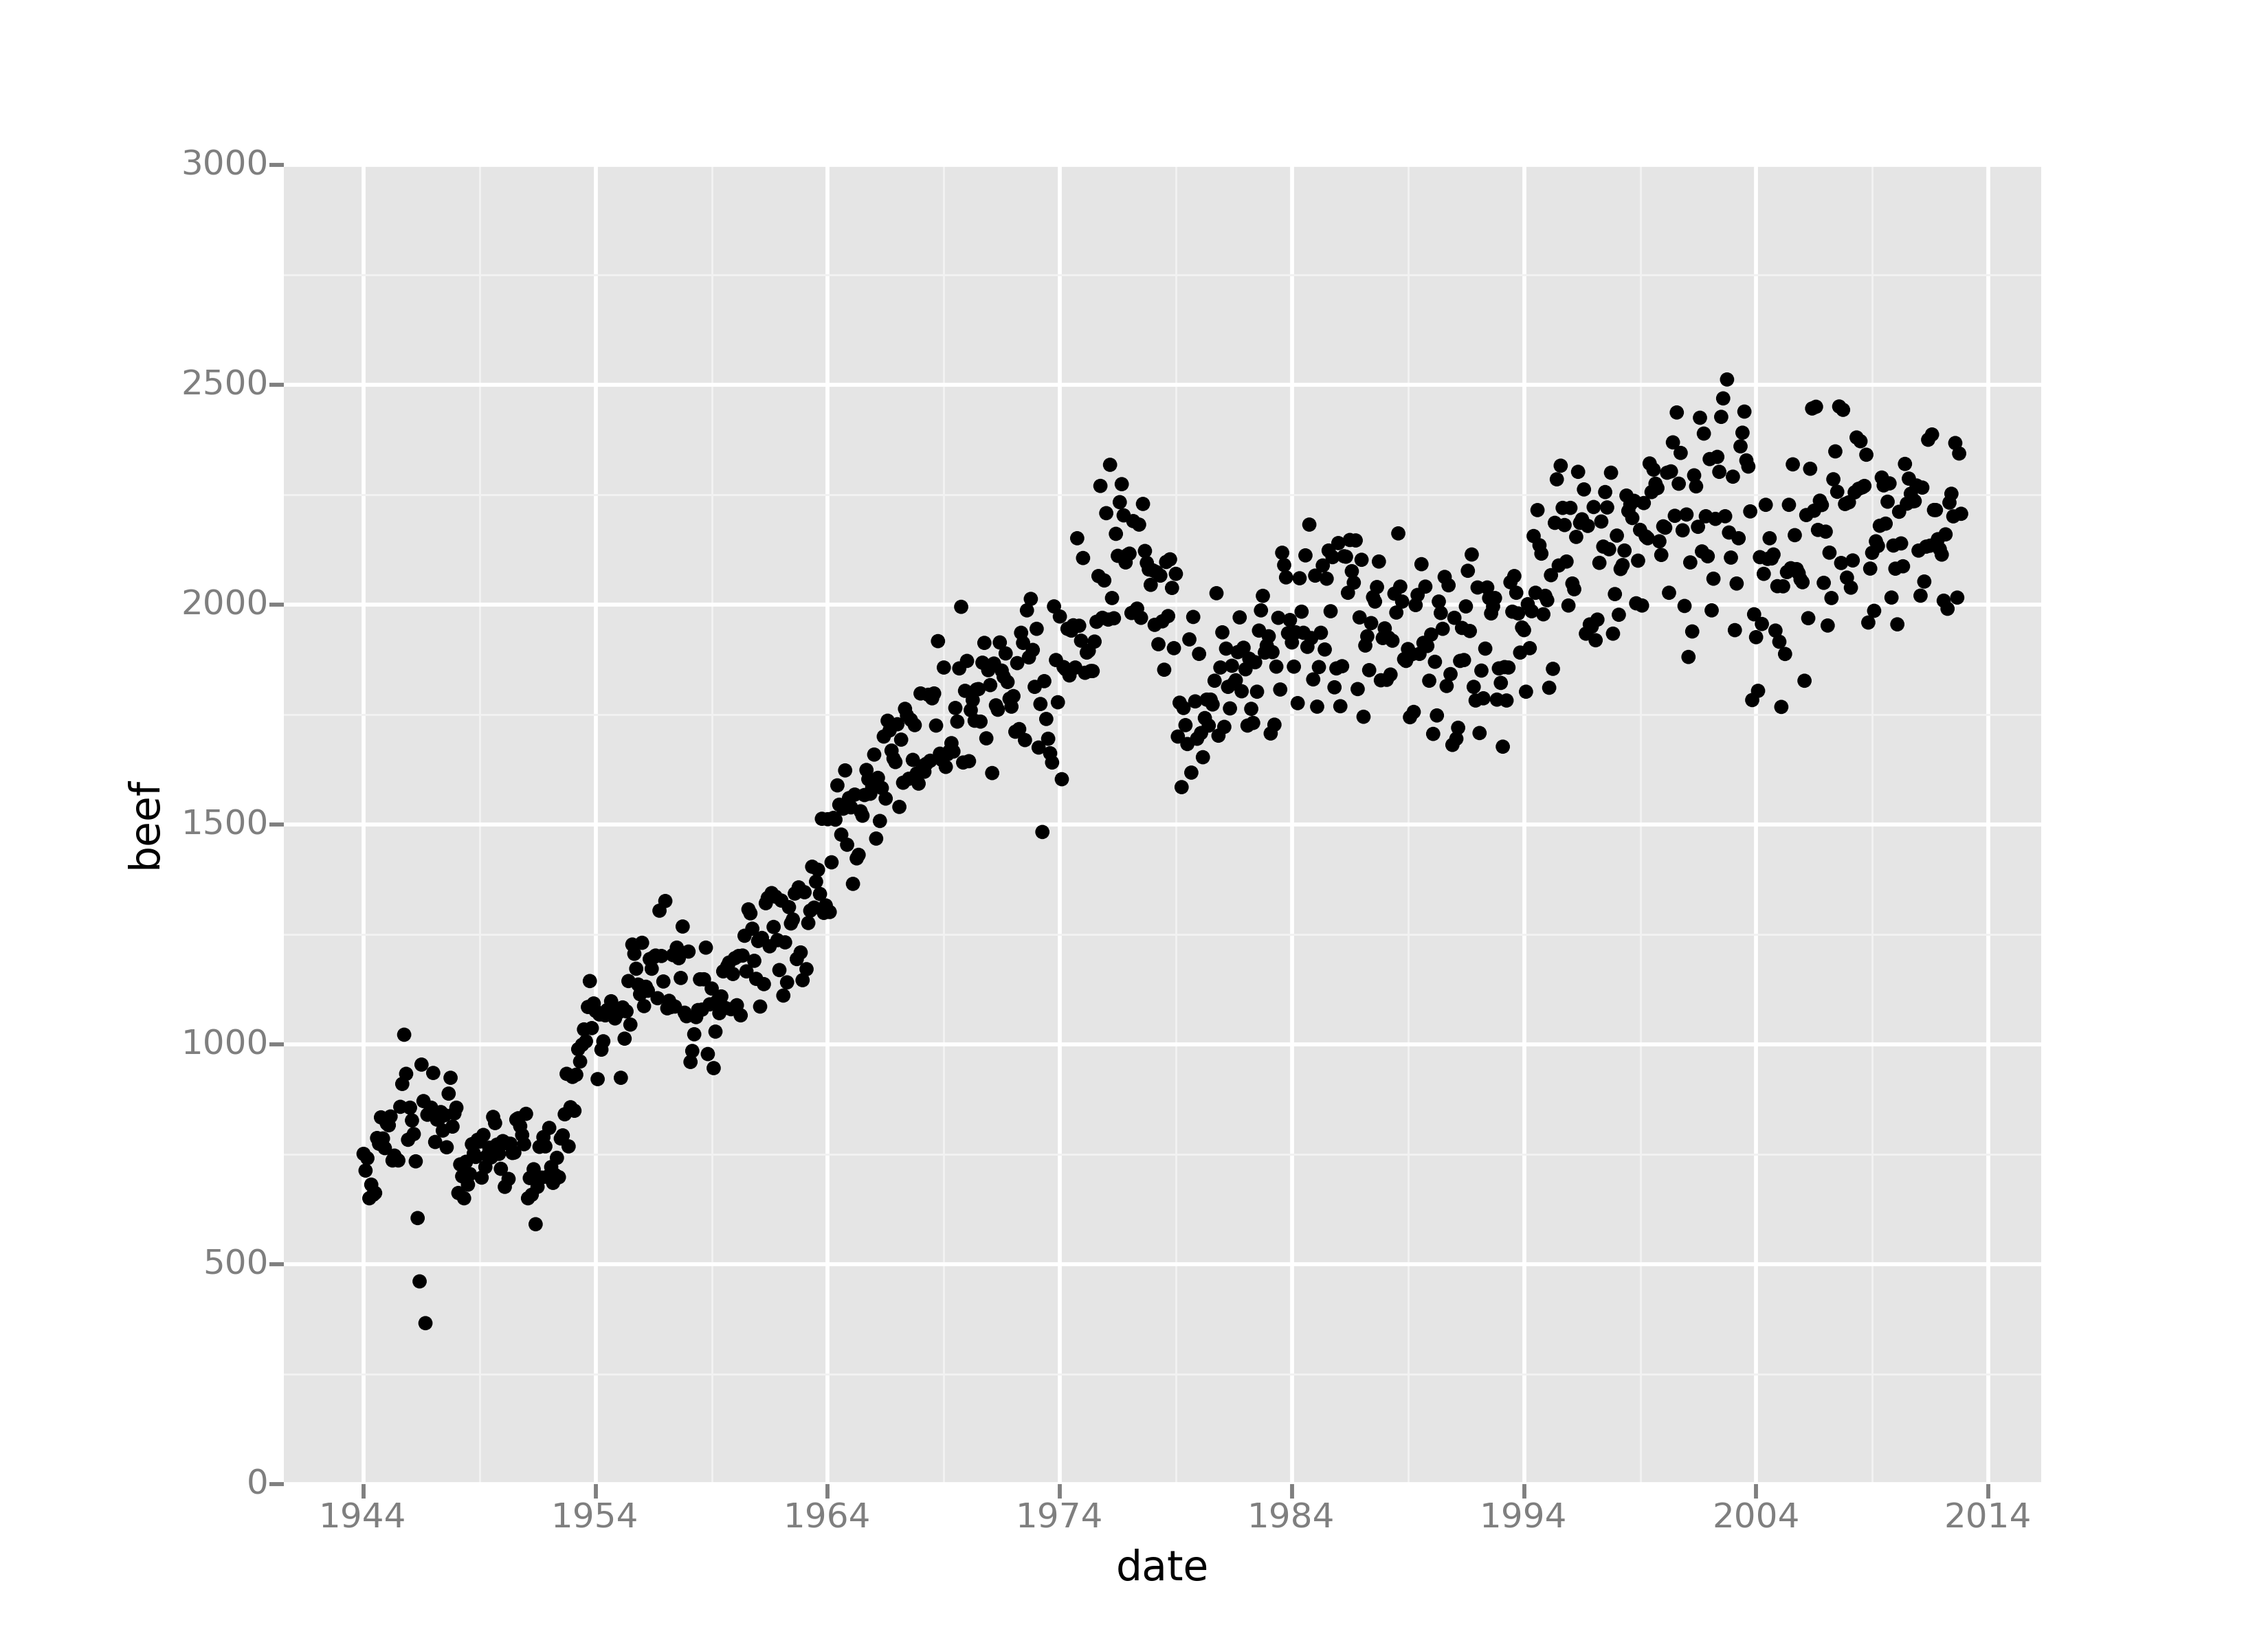
\includegraphics[width=0.7\linewidth]{Layers2}
			\end{figure}
	
	
\end{frame}
\begin{frame}[fragile]
Add a line.
	\begin{framed}
		\begin{verbatim}
p + geom_point() + geom_line()
		\end{verbatim}
	\end{framed}
	\begin{figure}
		\centering
		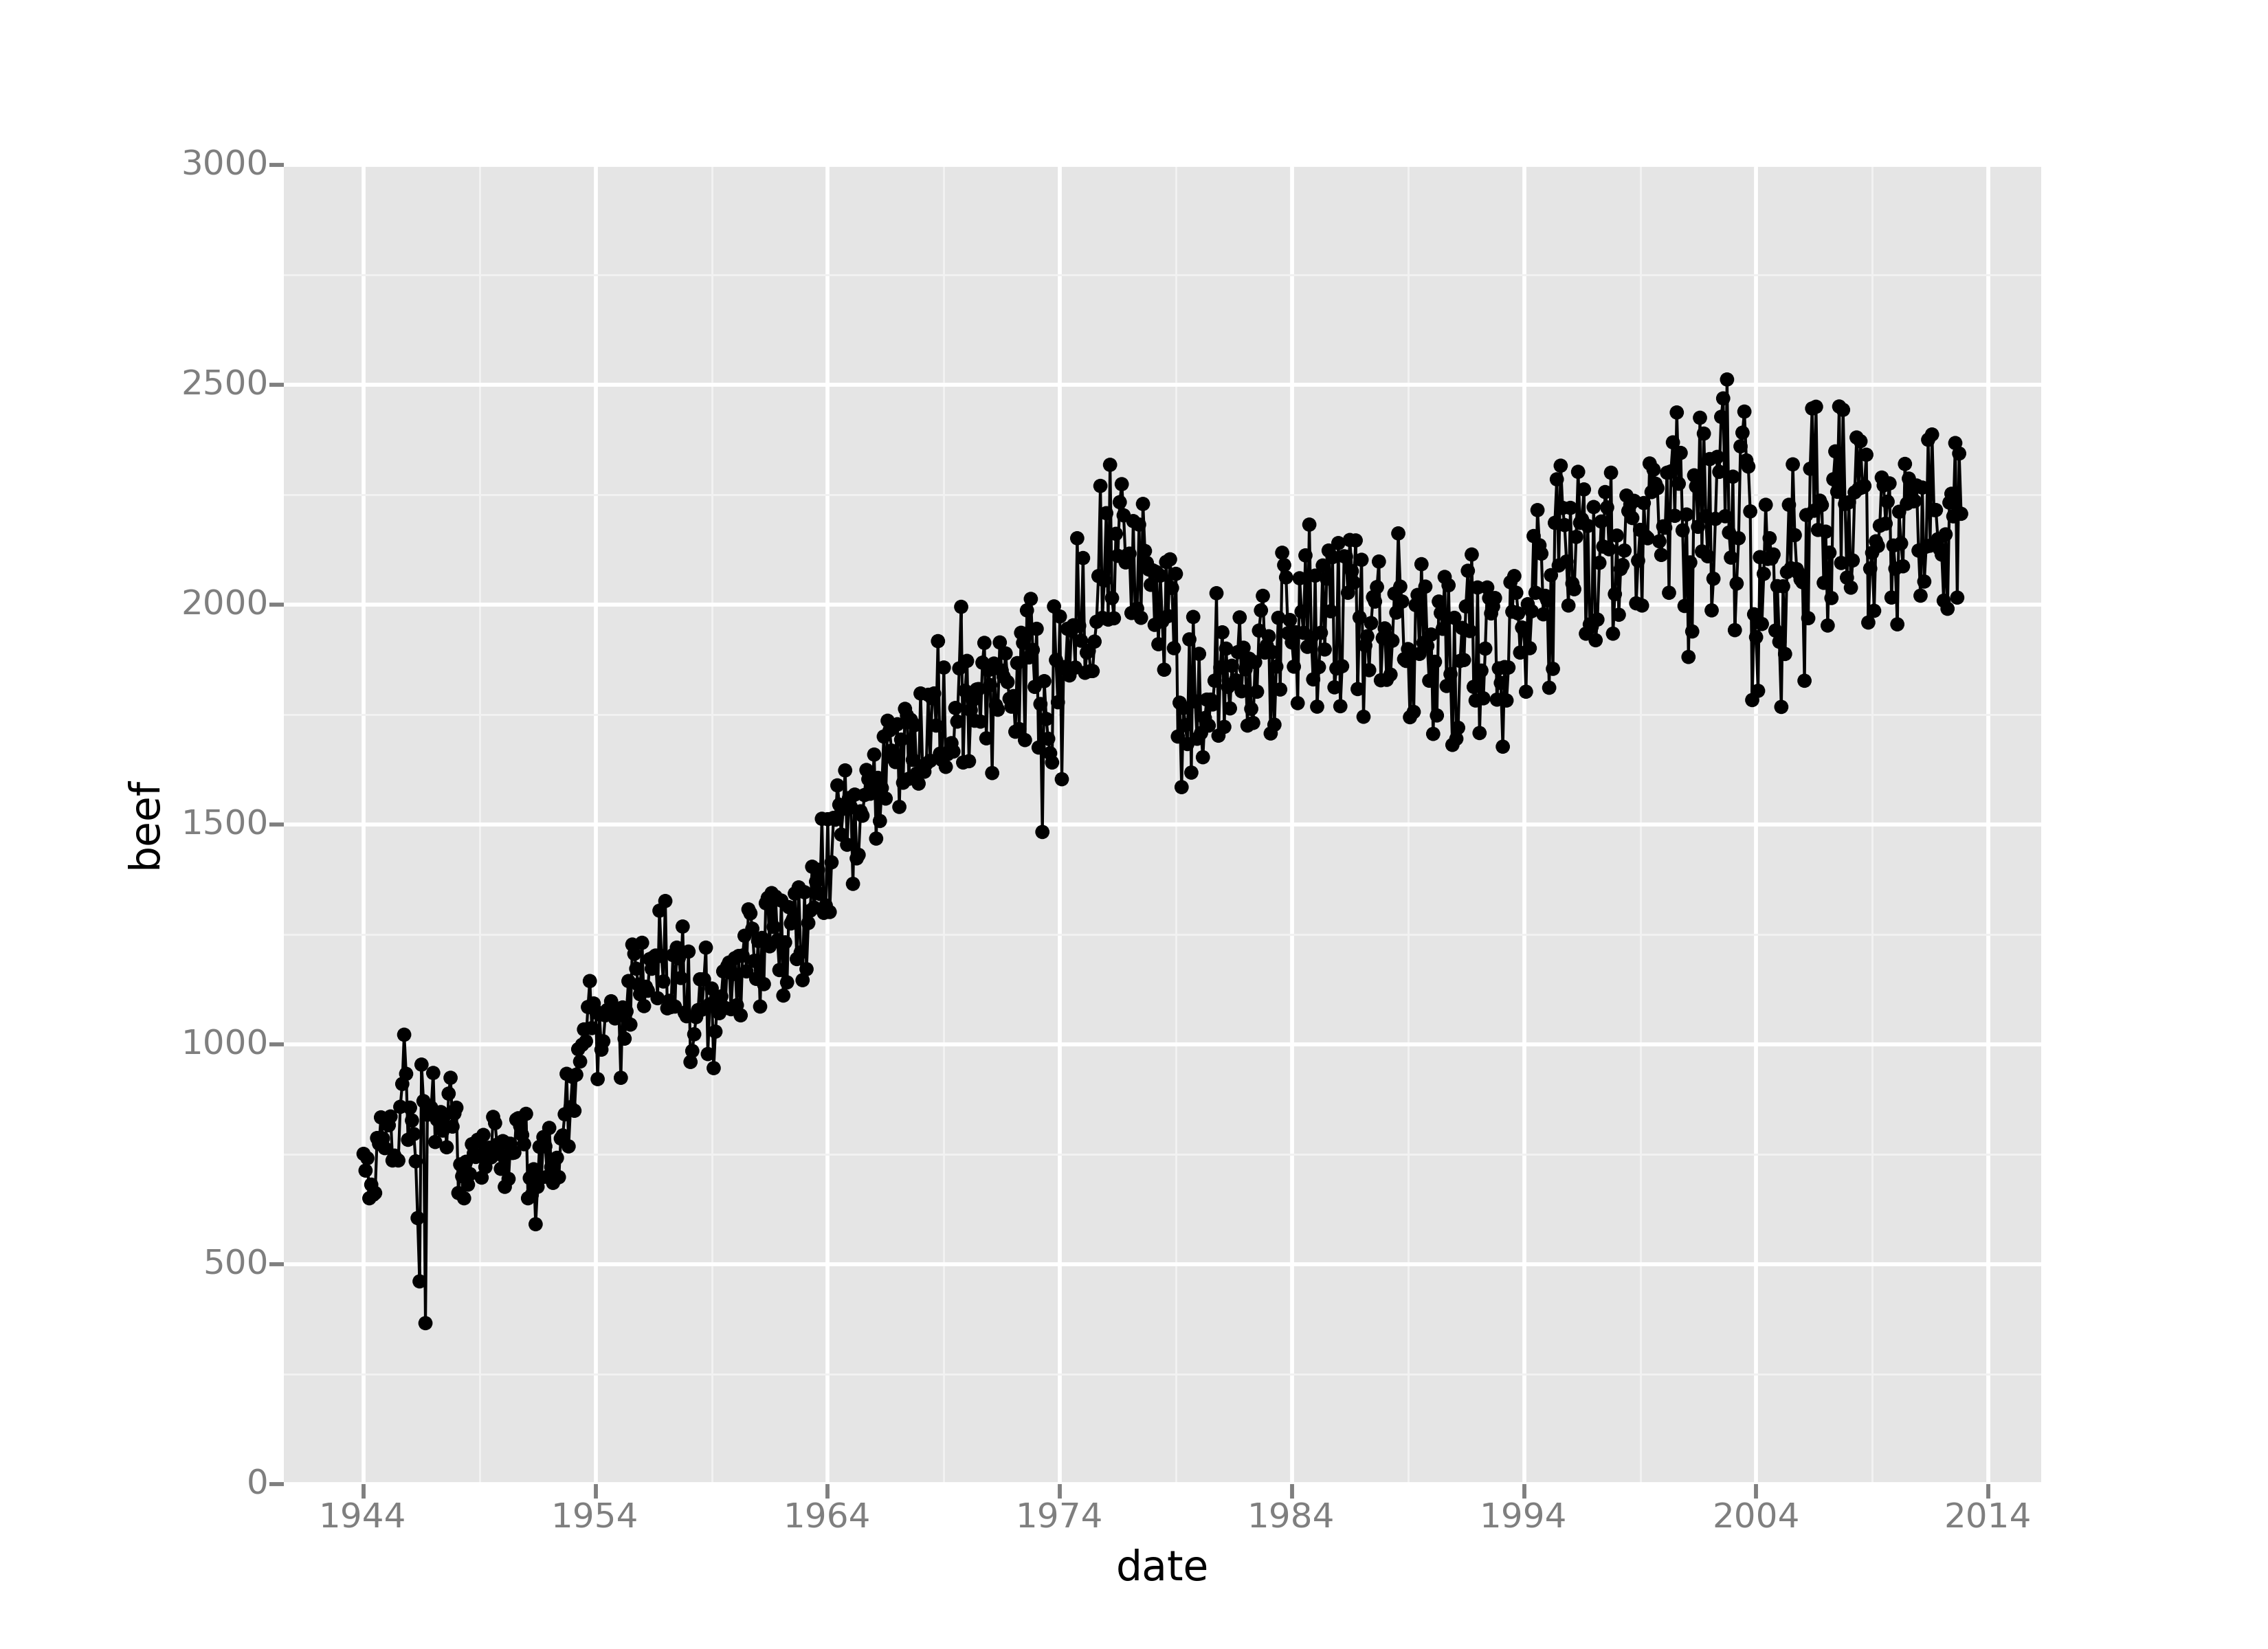
\includegraphics[width=0.7\linewidth]{Layers3}
	\end{figure}
	
	
\end{frame}





%================================================================================== %
\begin{frame}[fragile]
Add a trendline.
	\begin{framed}
\begin{verbatim}
p + geom_point() + geom_line() +
 stat_smooth(color="blue")
\end{verbatim}
\end{framed}
\begin{figure}
\centering
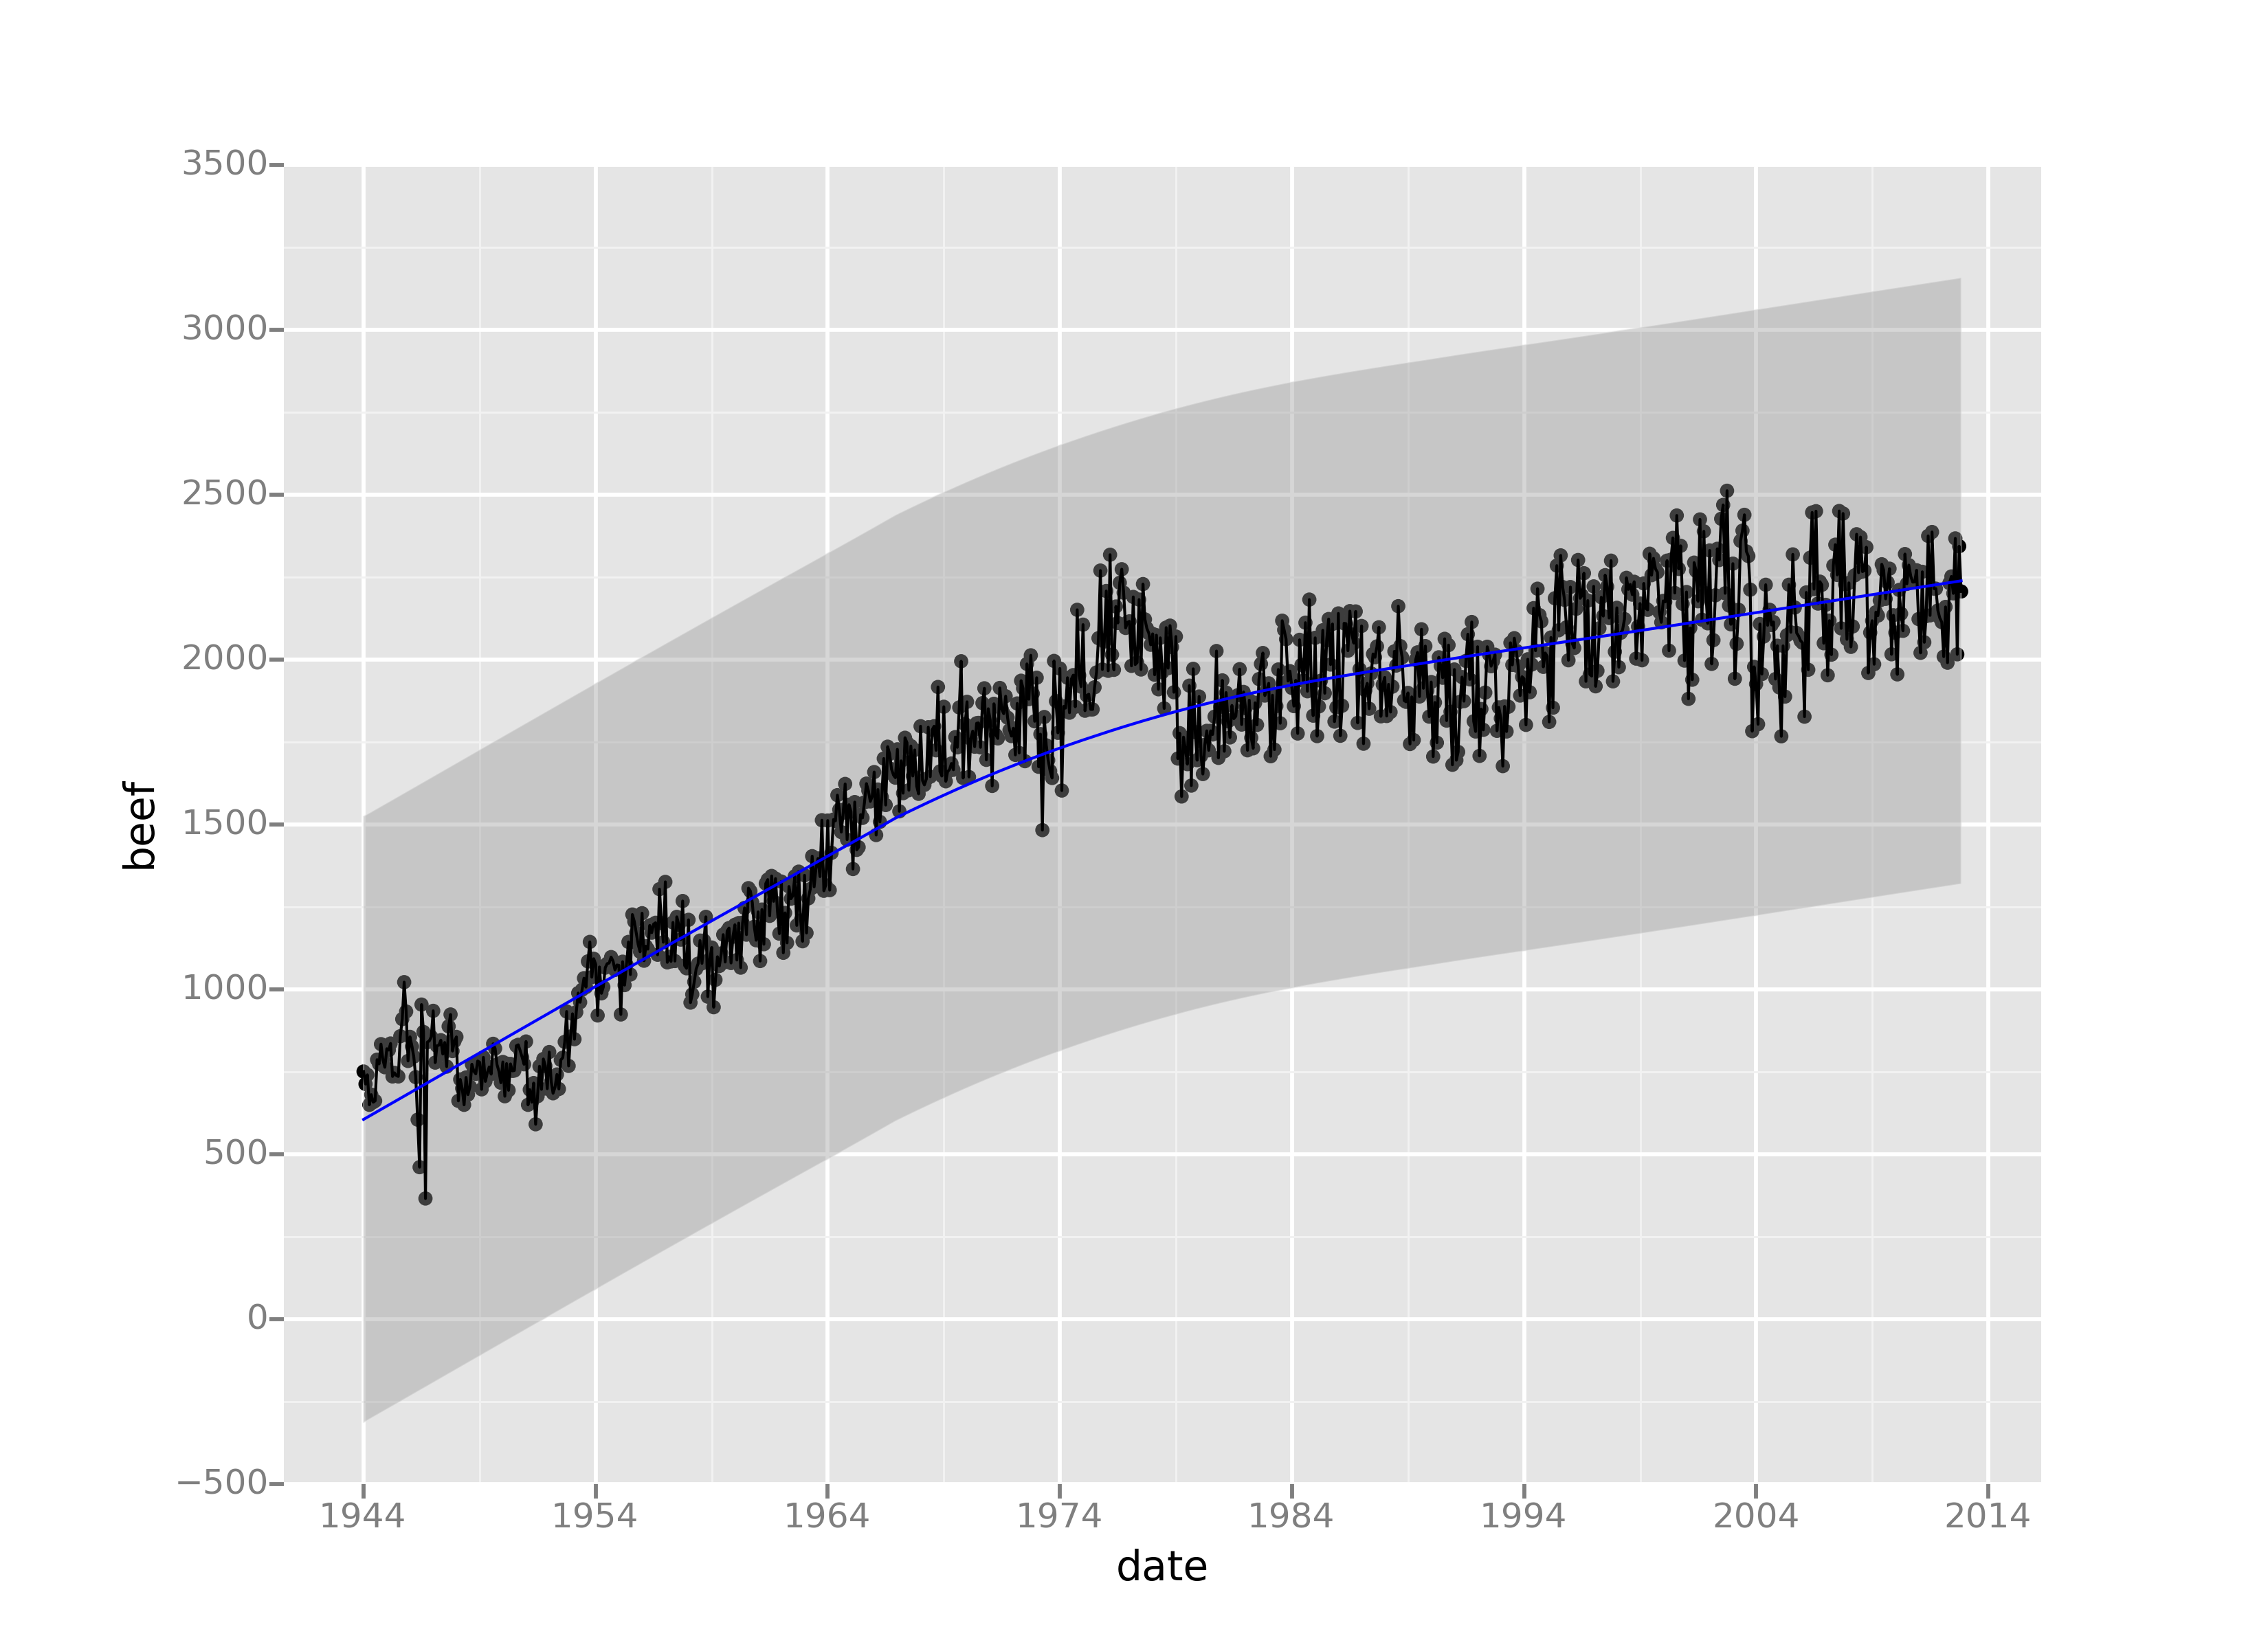
\includegraphics[width=0.7\linewidth]{layers4}
\end{figure}
\end{frame}
%================================================================================== %

\begin{frame}
	\Large
	Geometric objects (geoms) are the visual representations of (subsets of) observations.
\begin{itemize}
	\item \textbf{Univariate} - single numeric variable
	\item \textbf{Bivariate} - two numeric variable
	\item \textbf{Multivariate} - Multiple variables
\end{itemize}
\end{frame}
%============================== %
\begin{frame}
\Large
\noindent \textbf{Faceting}\\
	The faceting approach supported by ggplot2 partitions a plot into a matrix of panels. Each panel shows a different subset of the data.
	 There are two faceting approaches:
	
	\begin{itemize}
	\item \texttt{facet\_wrap($\sim$cell)} - univariate: create a 1-d strip of panels, based on one factor, and wrap the strip into a 2-d matrix
	\item \texttt{facet\_grid(row$\sim$col)} - (usually) bivariate: create a 2-d matrix of panels, based on two factors
	\end{itemize}
\end{frame}
%================================= %
%- http://sape.inf.usi.ch/quick-reference/ggplot2/scale
\begin{frame}
	\Large
	\noindent \textbf{Scales}
	\begin{itemize}
\item A scale determines how an attribute of the data is mapped into an aesthetic property of a geom (e.g., the geom's position along the x axis, or a geom's fill color in a color space).
	\end{itemize}

\end{frame}
\end{document}